\documentclass[a4paper]{report}

%====================== PACKAGES ======================

\usepackage[french]{babel}
\usepackage[utf8x]{inputenc}
%pour gérer les positionnement d'images
\usepackage{float}
\usepackage{amsmath}
\usepackage{graphicx}
\usepackage[colorinlistoftodos]{todonotes}
\usepackage{url}
%pour les informations sur un document compilé en PDF et les liens externes / internes
\usepackage{hyperref}
%pour la mise en page des tableaux
\usepackage{array}
\usepackage{tabularx}
%pour utiliser \floatbarrier
%\usepackage{placeins}
%\usepackage{floatrow}
%espacement entre les lignes
\usepackage{setspace}
%police et mise en page (marges) du document
\usepackage[T1]{fontenc}
\usepackage[top=2cm, bottom=2cm, left=2cm, right=2cm]{geometry}
%Pour les galerie d'images
\usepackage{subfig}
%Pour inclure du code\
\usepackage{listings}

%====================== INFORMATION ET REGLES ======================

%rajouter les numérotation pour les \paragraphe et \subparagraphe
\setcounter{secnumdepth}{4}
\setcounter{tocdepth}{4}

\hypersetup{							% Information sur le document
pdfauthor = {Sias Nicolas 2TL1,
			Mouton Youri 2TL2},			% Auteurs
pdftitle = {Langage avancée de programmation -
			Projet Java : GénialBall},			% Titre du document
pdfsubject = {GénialBall},		% Sujet
pdfkeywords = {GénialBall, projet, java, ...},	% Mots-clefs
pdfstartview={FitH}}					% ajuste la page à la largueur de l'écran
%pdfcreator = {MikTeX},% Logiciel qui a crée le document
%pdfproducer = {}} % Société avec produit le logiciel

%======================== DEBUT DU DOCUMENT ========================

\begin{document}

%régler l'espacement entre les lignes
\newcommand{\HRule}{\rule{\linewidth}{0.5mm}}

%page de garde
\begin{titlepage}
\begin{center}

% Upper part of the page. The '~' is needed because only works if a paragraph has started.
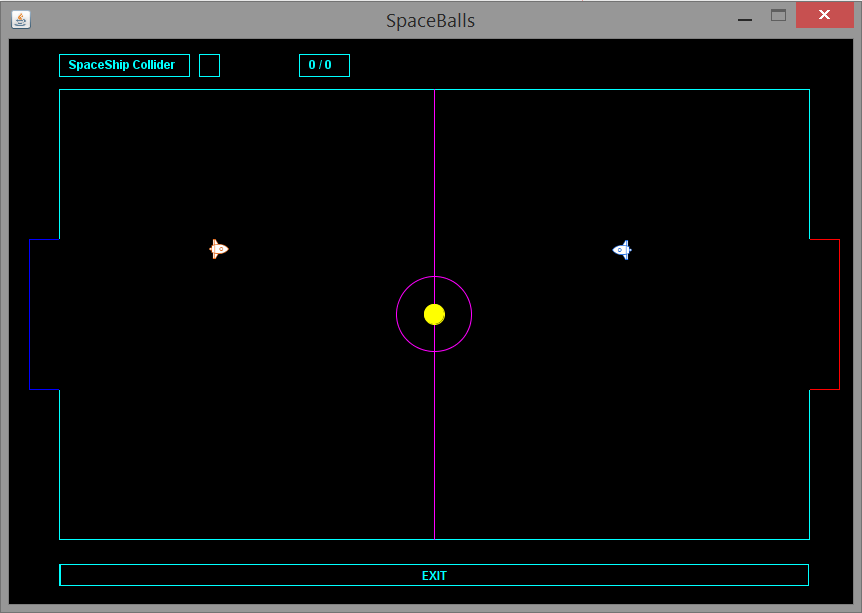
\includegraphics[width=15cm]{./TerrainAvecJoueur.png}~\\[1cm]

\textsc{\LARGE Langage avancé de programmation}\\[1.5cm]

\textsc{\Large }\\[0.5cm]

% Title
\HRule \\[0.4cm]
y
{\huge \bfseries Projet Java\\
GénialBall \\[0.4cm] }

\HRule \\[1.5cm]

% Author and supervisor
\begin{minipage}{0.4\textwidth}
\begin{flushleft} \large
\emph{Auteur:}\\
Nicolas Sias 2TL1\\
Youri Mouton 2TL2
\end{flushleft}
\end{minipage}
\begin{minipage}{0.4\textwidth}
\begin{flushright} \large
\emph{Année académique:} \\
2014-2015
\end{flushright}
\end{minipage}

\vfill

\end{center}
\end{titlepage}

%page blanche
\newpage
~
%ne pas numéroter cette page
\thispagestyle{empty}
\newpage

\tableofcontents
\thispagestyle{empty}
\setcounter{page}{0}
%ne pas numéroter le sommaire

\newpage

%espacement entre les lignes d'un tableau
\renewcommand{\arraystretch}{1.5}

%====================== INCLUSION DES PARTIES ======================

~
\thispagestyle{empty}
%recommencer la numérotation des pages à "1"
\setcounter{page}{0}
\newpage

\chapter{Introduction}

\section{Qu'est-ce que GénialBall ?}

GénialBall est un jeu de sport, dans un mélange de football et d’air-hockey, où deux joueurs s’affrontent en réseau local, ayant comme but de pousser le ballon dans le but adverse.\\

\section{Comment y jouer ?}

Lancez l'application, choississez d'être le client ou le serveur ( un joueur doit être le client, l'autre doit être le serveur), attendez que la recherche d'IP local se termine, puis selectionnez l'IP local de votre adversaire.
%inclusion d'une mage dans le document
\begin{figure}[!h]
\begin{center}
%taille de l'image en largeur
%remplacer "width" par "height" pour régler la hauteur
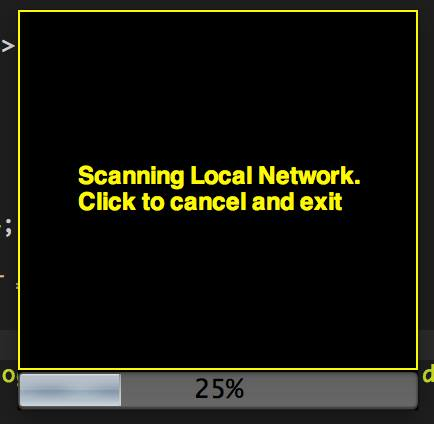
\includegraphics[width=5cm]{./ScanningNetwork}
%légende de l'image
\caption{Le jeu va d'abord chercher les autres machines connectées dans le réseau local.}
\end{center}
\end{figure}

\begin{figure}[!h]
\begin{center}
%taille de l'image en largeur
%remplacer "width" par "height" pour régler la hauteur
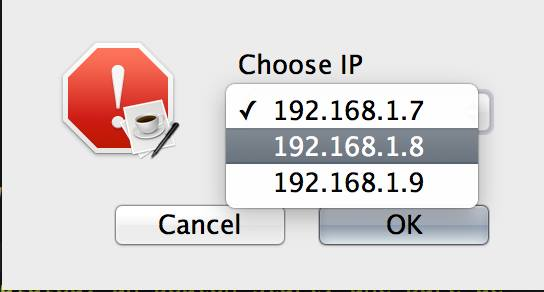
\includegraphics[width=5cm]{./ChooseYourIp}
%légende de l'image
\caption{Sélectionnez ensuite l'IP local de votre adversaire}
\end{center}
\end{figure}

\newpage

\section{Interface du jeu}
%inclusion d'une mage dans le document
\begin{figure}[!h]
\begin{center}
%taille de l'image en largeur
%remplacer "width" par "height" pour régler la hauteur
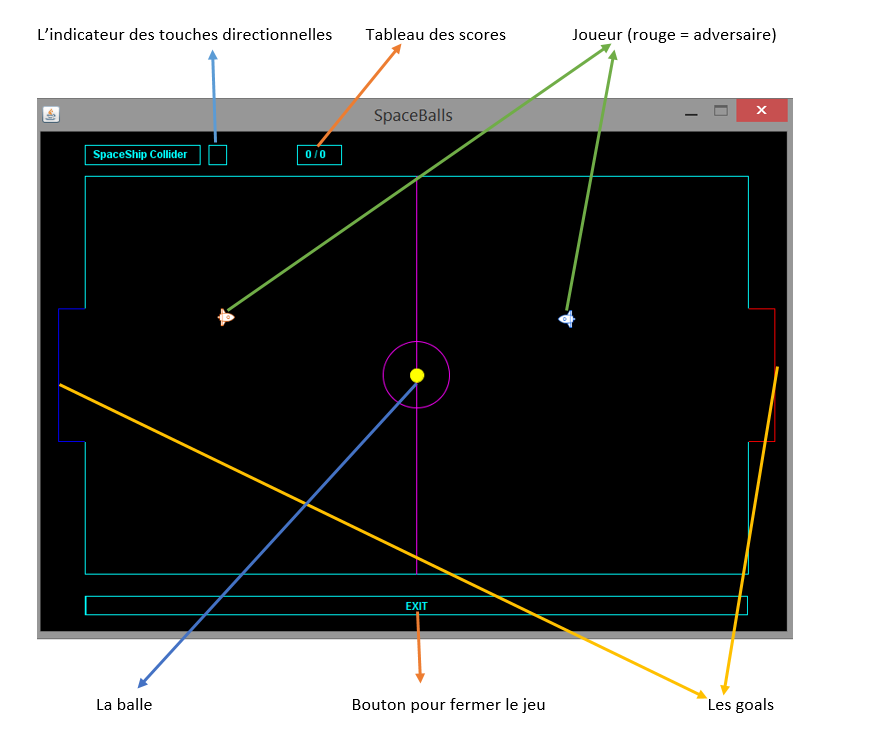
\includegraphics[width=20cm]{./InterfaceGraph}
\end{center}
\end{figure}

\section {Les contrôles du jeu}

\begin{itemize}
\item Utilisez les touches directionnelles pour déplacer votre vaisseau.
\item Appuyez sur la barre d'espace si vous désirez faire un tir avec la balle.
\item Si vous désirez quitter, cliquez sur la touche "Exit" ou appuyez sur Esc.
\end{itemize}



\chapter{Extrait UML}

\begin{figure}[!h]
\begin{center}
%taille de l'image en largeur
%remplacer "width" par "height" pour régler la hauteur
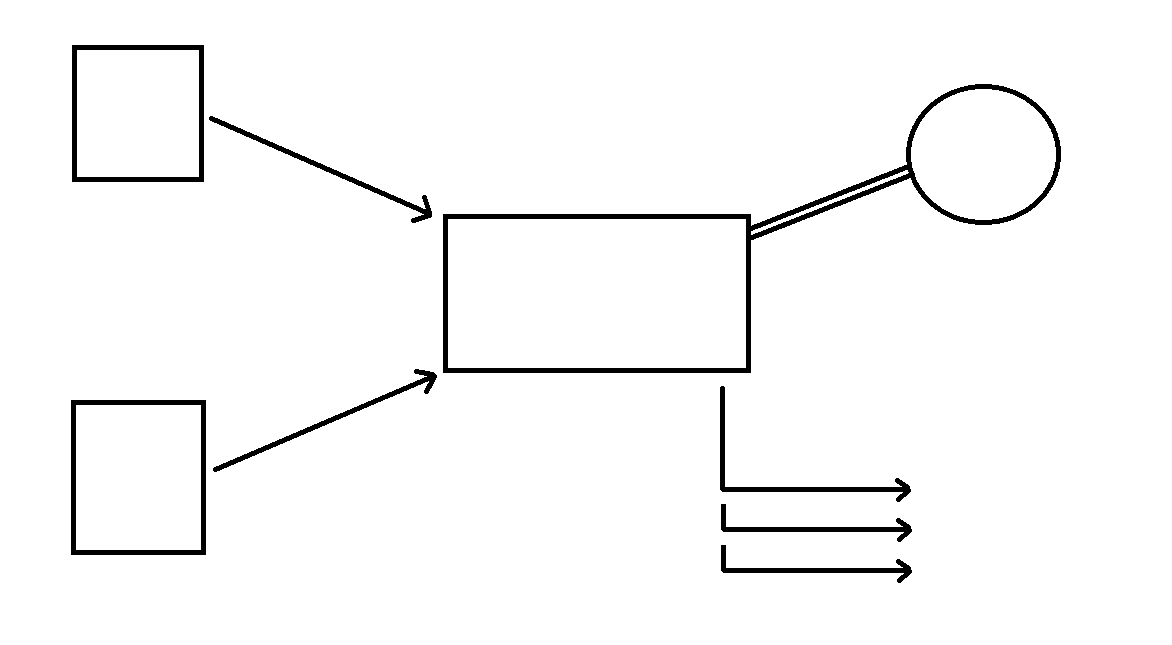
\includegraphics[width=15cm]{presentation/schema}
\end{center}
\caption{Extrait UML des classes joueur}
\end{figure}

 
\chapter{Extrait du code source (SpaceBalls.java)}

\lstset{language=Java}
\begin{lstlisting}
package main;

import gui.Board;

import java.awt.EventQueue;

import javax.swing.JFrame;

@SuppressWarnings("serial")
public class SpaceBalls extends JFrame {

	Board mainBoard;

	public SpaceBalls() throws Exception {
		// our main window is 850x600 for now.
		this.setSize(850, 600);

		// initialize a board which takes the whole screen
		mainBoard = new Board(this.getSize());

		// add the jpanel in the jframe
		add(mainBoard);

		// jframe settings
		this.setTitle("SpaceBalls");
		this.setResizable(false);
		this.setDefaultCloseOperation(JFrame.EXIT_ON_CLOSE);
		this.setLocationRelativeTo(null);

	}

	public static void main(String[] args) {
		// main loop
		EventQueue.invokeLater(new Runnable() {
			// main application
			@Override
			public void run() {
				try {
					SpaceBalls ex = new SpaceBalls();
					ex.setVisible(true);
				} catch (Exception e) {
					e.printStackTrace();
				}}});}}

\end{lstlisting}

\chapter{Documentation JavaDoc HTML}

Toute la javaDoc est dans un fichier annexe "doc". Si vous désirez lire notre javaDoc, veuillez selectionner dans ce fichier "index.html"

\begin{figure}[!h]
\begin{center}
%taille de l'image en largeur
%remplacer "width" par "height" pour régler la hauteur
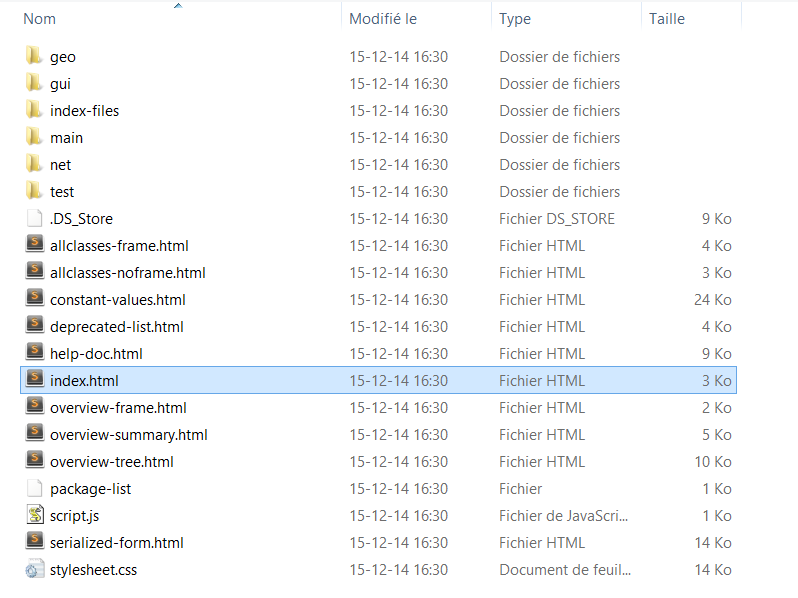
\includegraphics[width=15cm]{./javadocIllustration}
\end{center}
\end{figure}

\chapter{Description de votre stratégie de validation}

\section{Utilisation d'un package test}

Pour tester les points importants de notre jeu, nous avons créé plusieurs classes "test" dans un package mis à l'écart. Voici le contenu du package "test" :

\paragraph*{ClientTest.java :}
Cette classe sert à détecter les erreurs de réception et/ou d'envoi de chaînes de caractères au serveur.  

\paragraph*{ExitButtonTest.java :} Elle sert à vérifier si le bouton "Exit" lorsque le joueur 2 quitte la partie fonctionne.

\paragraph*{FieldTest.java :} Elle sert à détecter des erreurs lors de l'initialisation du Field, en liant le contrôle au visuel, utilisant du JUnit Testing

\paragraph*{InetTest.java :} Elle vérifie la détection de l'IP local par java (et savoir, par la même occasion, l'IP local du joueur lançant cette application).


\paragraph*{SwingWorkerTest :} Elle teste la recherche d'IP local (donc la classe DiscoverLocal.java).

\paragraph*{TextFieldTest :} Cette classe, utilisant le JUnit Testing, vérifie si l'affichage textuelle sur le terrain fonctionne. 

\section{JUnit Testing :}

On a utilisé le JUnit Testing principalement pour l'affichage textuelle sur le terrain ( via la classe TextFieldTest) ainsi que pour l'initialisation du terrain, en liant le contrôle au visuel (via la classe FieldTest)

\section{System.out.println}

Cette méthode a été utilisé très fréquemment pour détecter les collisions entre les objets (balle, terrain et joueur) .

\chapter{Conclusion}

De manière générale, la conception de ce jeu nous a permis d'apprendre beaucoup sur l'Orienté Object appliqué à un projet avoisinant les 3000 lignes de code et les design patterns tels que le MVC.\\

Les gestions de collisions avec la balle a posé beaucoup de problèmes, la classe Ball.java a été réécrite plusieurs fois.\\ 

Le projet a permis une bonne introduction à la programmation évenementielle, aux éléments d'interface graphique et au threading, qui a permis de lancer nos processus jeu, serveur et client de manière concurrente sans bloquer les éléments d'interface graphique.\\

La manière dont le programme envoie les informations pourrait être fort améliorée, utiliser UDP permetterait de pouvoir jouer sans que le déplacement des joueurs et de la balle soit saccadé.\\

Nous utilisons une boite de dialogue avec une barre de progrès lorsque le programme essaye de trouver des ordinateurs connectés sur le réseau local, nous pourrions lancer une requète UDP en broadcast pour ne trouver que les ordinateurs qui ont un ServerSocket écoutant sur un port qui nous intéresse.\\

L'utilisation d'une librairie graphique aurait pu nous faciliter la tâche et nous permettre de nous concentrer sur d'autres aspects et détails du jeu, mais ce fut un apprentissage intéressant.\\

Le programme manque d'un panneau de configuration graphique que l'on aurait bien voulu coder, mais le temps donné ne nous l'a pas permis.\\


\end{document}